%!TEX root = A0.Master.tex
\chapterbegin{Descripción de la aplicación: cliente y servidor}

La aplicación desarrollada en el presente proyecto está compuesta por dos partes fundamentales: el proveedor de datos situado en un servidor remoto, y la aplicación del dispositivo móvil, que pide datos al servidor e interpreta en la pantalla del usuario dichos resultados.

Como ya se ha comentado en el primer capítulo, la parte del servidor no será descrita por completo ya que no entra dentro del ámbito de este Proyecto de Fin de Carrera.

\section{Cliente}
En esta sección nos concentraremos en describir la aplicación cliente que el usuario dispondrá en su iPhone. Este cliente debe proporcionar de manera rápida y eficaz la información que necesita el usuario. Para ello se ha diseñado un sistema de navegación de varios pasos consecutivos, simplificando la UI al máximo para cumplir los requisitos de rapidez y eficacia, teniendo en mente siempre que el usuario utilizará nuestra aplicaciones por un tiempo menor de 30 segundos, ya que se encuentra ocupado comprando en la tienda física. En la figura \ref{fig:esqueleto} se muestra el esqueleto de nuestra aplicación cliente.

\begin{figure}[h]
	\centering
		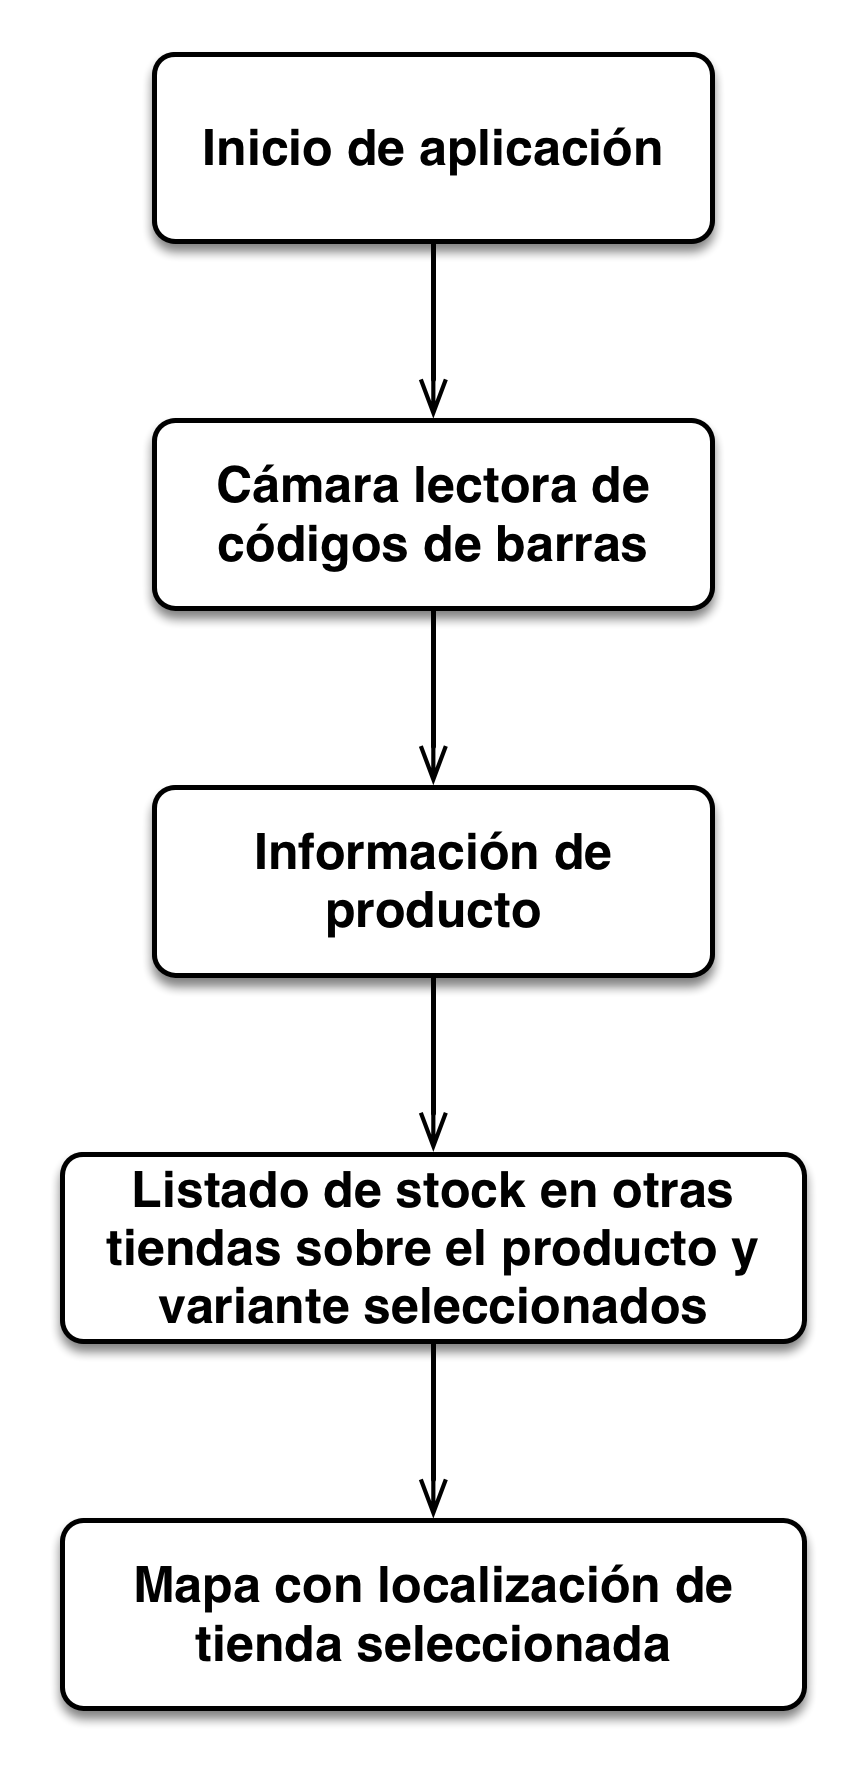
\includegraphics[width=0.3\textwidth]{./img/esqueleto-app.png}
	\caption{Esqueleto de navegación entre pantallas de la aplicación móvil cliente del usuario.}
	\label{fig:esqueleto}
\end{figure}

\subsection{Pantallas del cliente}
 
\subsubsection{Pantalla de inicio: cámara}

\subsubsection{Pantalla de información de producto}

\subsubsection{Pantalla de lista de tiendas con stock}

\subsubsection{Pantalla de mapa con tienda geolocalizada}

\subsection{Petición y recepción de datos del servidor en el cliente}
Como ya se ha comentado anteriormente, la aplicación cliente realiza peticiones al servidor, que devuelve los datos en formato JSON.

\section{Servidor}

\chapterend